% Tipo de documento a utilizar
\documentclass[12pt, a4paper, twoside, openright, english]{book}
%Idioma e tipo de escrita (encriptacao latina)
\usepackage[english]{babel}
%\usepackage[
%singlelinecheck=false % <-- important
%]{caption}

\usepackage[xetex]{graphicx}
\usepackage{fontspec,xunicode}
\setmainfont[ AutoFakeSlant=0.15 ]{NewsGotT}

\renewcommand{\baselinestretch}{1.25cm}
% Identacao no primeiro paragrafo
\usepackage{indentfirst}

%simbolos matematicos
\usepackage{amssymb}

%Espaçamento
\usepackage[onehalfspacing]{setspace}

%Margens do documento
\usepackage[inner=2.5cm,outer=2.5cm,top=2.5cm, bottom=2.5cm, headheight=20pt, headsep=0.75cm]{geometry}

%rotacao de figuras para a horizontal
\usepackage{pdflscape}

%\usepackage{rotating}

%Tipo de letra, cabeçalhos, tabela de conteúdos, equações e referências
\usepackage{ fancyhdr, amsmath, textcomp, array, booktabs} %, cite} \bibliographystyle{unsrt}
%Estilo da bibliografia e modos operandi

\usepackage[square, sort&compress, numbers]{natbib}
\bibliographystyle{unsrtnat}

\usepackage{notoccite} % nao considerar a lista de figuras e tabelas para construcao das referencias
\usepackage[nottoc]{tocbibind} %- remove o índice do hyperef

%Configuração das tabelas
%\setlength{\tabcolsep}{3pt}
\usepackage{caption, multirow}
\usepackage[table, xcdraw, color]{xcolor}

\usepackage{geometry}
\usepackage{pdflscape} % rotacao de tabelas 
\captionsetup[table]{skip=6pt}
\usepackage{chngcntr}
\counterwithout{figure}{chapter}
\counterwithout{table}{chapter}
\counterwithout{equation}{chapter}
%Lista de itens
\usepackage[shortlabels]{enumitem}
\setlist[enumerate]{nosep}

%PACKAGE PARA ADICIONAR FICHEIROS PDF (CAPA)
\usepackage[final]{pdfpages}

%Alterar o comportamento das imagens
%\usepackage{graphicx, float, subcaption, epstopdf, morefloats, multicol}
\usepackage{graphicx, float, subcaption, morefloats, multicol}
\graphicspath{ {images/} }

%Estilo dos Capítulos
\usepackage[Lenny]{fncychap}

%Apagar o que fica entre capítulos
\let\origdoublepage\cleardoublepage
\newcommand{\clearemptydoublepage}{%
  \clearpage
  {\pagestyle{empty}\origdoublepage}%
}

% Modo de referência das figuras
\newcommand{\fref}[1]{Figure~\ref{#1}}
\newcommand{\tref}[1]{Table~\ref{#1}}
\newcommand{\eref}[1]{(\ref{#1})}
\newcommand{\cref}[1]{Chapter~\ref{#1}}
\newcommand{\sref}[1]{Section~\ref{#1}}
\newcommand{\aref}[1]{Appendix~\ref{#1}}

\usepackage{boldline}
%Incluir subsecções na tabela de conteúdos
\setcounter{secnumdepth}{3}
\setcounter{tocdepth}{3}

% Criacao de links para o pdf
\usepackage[bookmarksnumbered=true, hidelinks]{hyperref}
 
%Listagem de figuras e tabelas no TABLE od CONTENTS
\renewcommand{\listoffigures}{\begingroup
\tocsection
\tocfile{\listfigurename}{lof}
\endgroup}

%Package para acrónimos e nomenclaturas
\usepackage[acronym, toc]{glossaries}
\usepackage{amsmath}
\DeclareMathOperator{\mtt}{MTT}
\DeclareMathOperator{\rcbv}{rCBV}
\DeclareMathOperator{\rcbf}{rCBF}
\DeclareMathOperator*{\argmax}{arg\,max}
\DeclareMathOperator{\softmax}{softmax}
\DeclareMathOperator{\dist}{d}
\DeclareMathOperator{\EX}{\mathbb{E}}

\usepackage{soul,color}
\DeclareRobustCommand{\hlcyan}[1]{{\sethlcolor{cyan}\hl{#1}}}
\soulregister\cite7
\soulregister\citet7
\soulregister\ref7
\soulregister\pageref7
\soulregister\acrshort7
\soulregister\textsubscript7
\usepackage{textcomp}
\newacronym{ml}{ML}{Machine Learning}



\makeglossaries

%APENDICES
\usepackage[titletoc]{appendix} % \usepackage[titletoc, page]{appendix}

% alteracao do nome da tabela dos conteúdos
%\addto\captionsportuguese{% Replace "portuguese" with the language you use
 % \renewcommand{\contentsname}%
   % {Índice}%
%}
\usepackage{arydshln}
\usepackage{pifont}% http://ctan.org/pkg/pifont
\newcommand{\cmark}{\ding{51}}%
\newcommand{\xmark}{\ding{55}}%

% Para colocar paragraph com numeração e no index
\usepackage{titlesec}
\setcounter{secnumdepth}{4}
\setcounter{tocdepth}{4}
\titleformat{\paragraph}
{\normalfont\normalsize\bfseries}{\theparagraph}{1em}{}
\titlespacing*{\paragraph}
{0pt}{3.25ex plus 1ex minus .2ex}{1.5ex plus .2ex}

% Para espaçar as legendas de sub-imagens
\usepackage{subcaption}
\newlength{\imagewidth}

% Para fazer listings
\usepackage{listings}

\begin{document}
\selectlanguage{english}
	
	%CAPA DA TESE
	%ELIMINAR AS MARGENS
	\newgeometry{inner=0in,outer=0in,top=0in, bottom=0in}
	%\includepdf[pages=1]{chapters/contracapa_final_final_final.pdf}
	%\includepdf[pages=1]{chapters/CAPA-Dissertacao-Mestrado-EE.pdf}	
	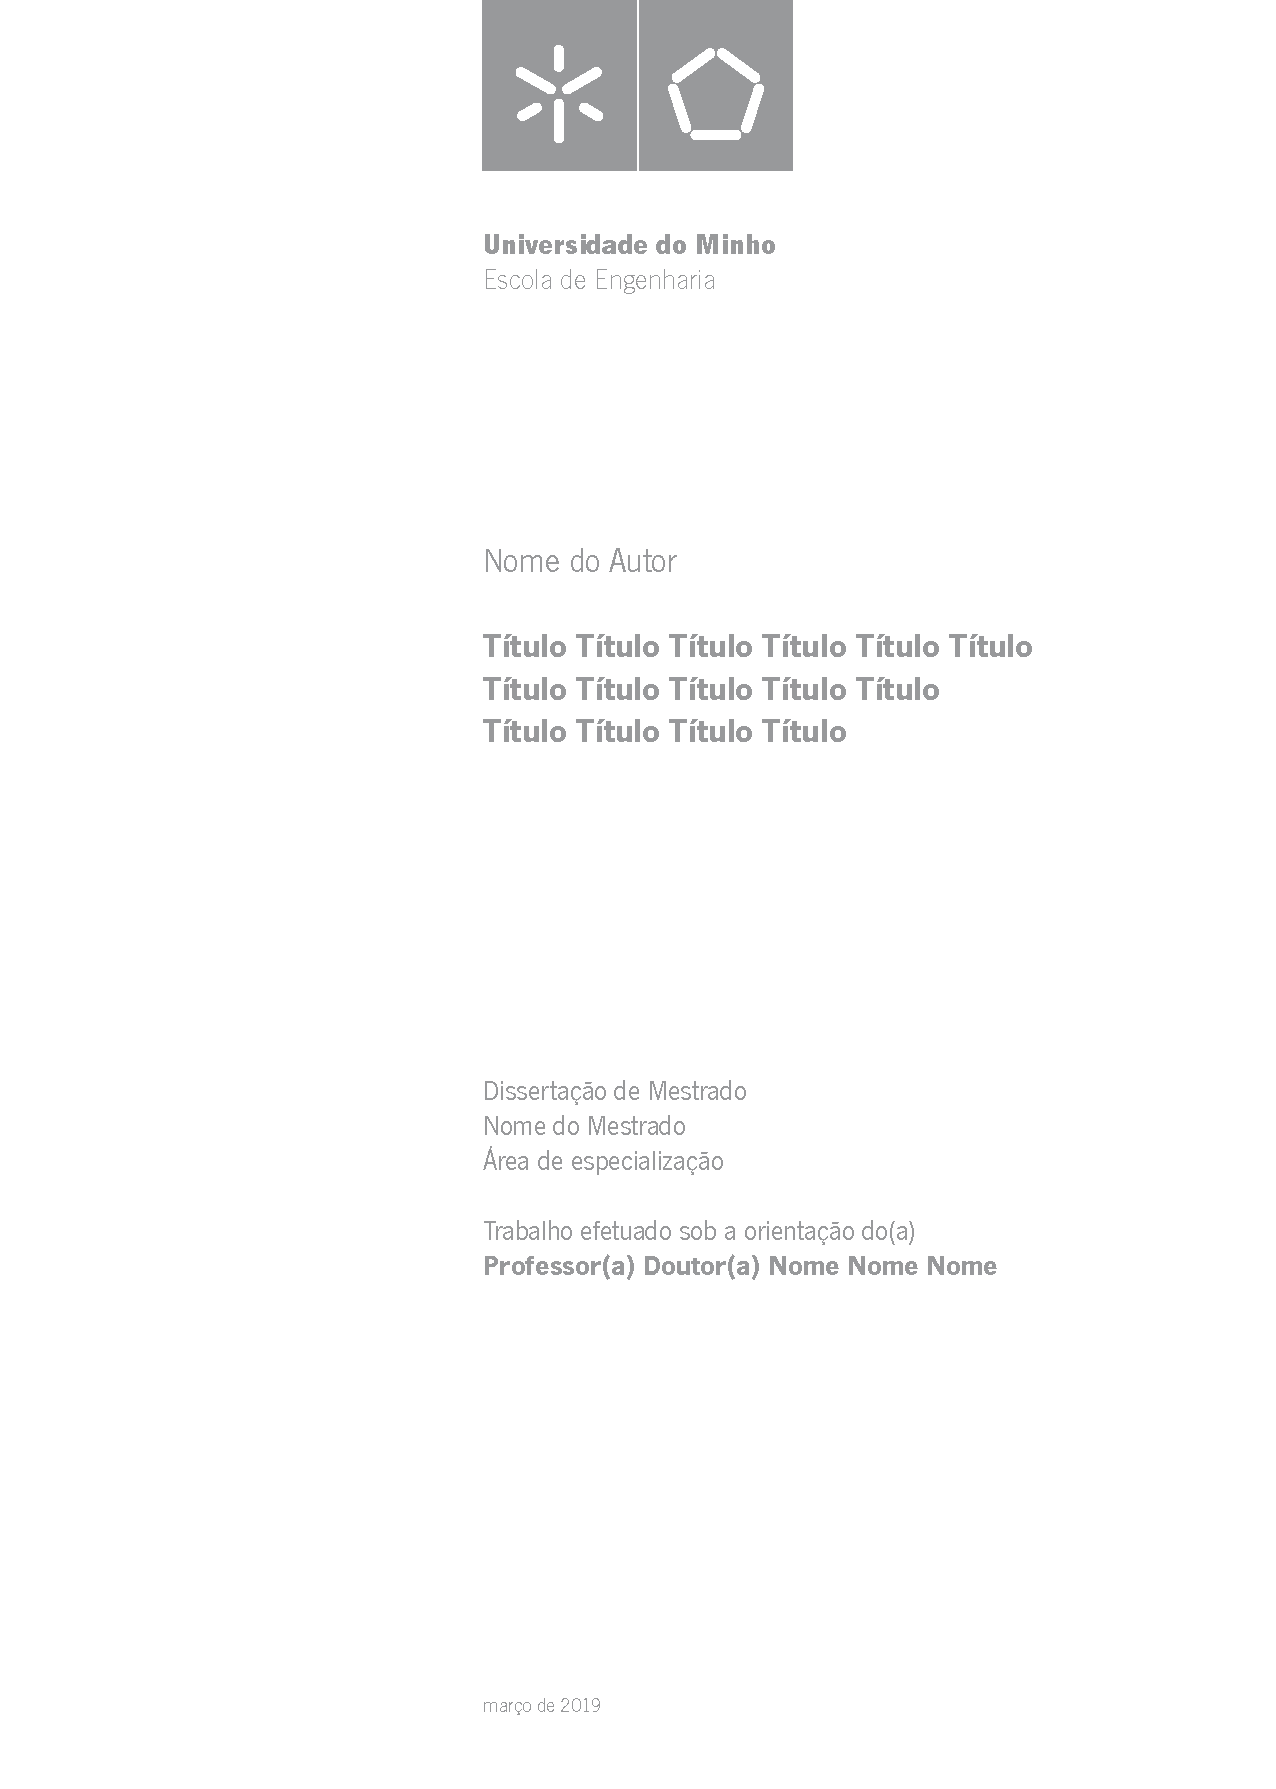
\includepdf[pages=1]{chapters/FOLHA-ROSTO-EE.pdf}	
	\restoregeometry
	
	% Numeração dos listings apenas com o seu número
	\renewcommand{\thelstlisting}{\arabic{lstlisting}}

	\let\cleardoublepage\clearpage

	%PÁGINAS INICAIS
	\frontmatter

	%HEADER E FOOT
	\pagestyle{plain}	
	
	%COPYRIGHTS
	\chapter{Direitos de Autor e Condições de Utilização do Trabalho por Terceiros}

Este é um trabalho académico que pode ser utilizado por terceiros desde que respeitadas as regras e
boas práticas internacionalmente aceites, no que concerne aos direitos de autor e direitos conexos.

Assim, o presente trabalho pode ser utilizado nos termos previstos na licença abaixo indicada.

Caso o utilizador necessite de permissão para poder fazer um uso do trabalho em condições não previstas
no licenciamento indicado, deverá contactar o autor, através do RepositóriUM da Universidade do Minho.

\textit{\textbf{Licença concedida aos utilizadores deste trabalho}}

\begin{figure}[H]
    
\includegraphics[width=0.15\textwidth]{copyrights.png}
\end{figure}

\vspace{-0.5cm}

\noindent\textbf{Atribuição}

\noindent\textbf{CC BY}

\noindent\url{https://creativecommons.org/licenses/by/4.0/}
	
	
	%AGRADECIMENTOS
	\chapter{Acknowledgments}

Your text here 

\begin{flushright}
Name
\end{flushright}

    %DECLARACAO INTEGRIDADE
	\pagestyle{plain}	
    \chapter{Statement of Integrity}

I hereby declare having conducted this academic work with integrity. I confirm that I have not used
plagiarism or any form of undue use of information or falsification of results along the process leading to
its elaboration.

I further declare that I have fully acknowledged the Code of Ethical Conduct of the University of Minho.
	

	%RESUMO
	\chapter{Resumo}
\begin{center}
\textbf{Título da Dissertação}
\end{center}

Texto - Máximo uma página \newline

\textbf{Palavras-Chave: Máximo 5, ordenadas alfabeticamente}

	\chapter{Abstract}
\begin{center}
\textbf{Title of the Dissertation}
\end{center}

Text - Maximum one page \newline

\textbf{Keywords: Maximum 5, alphabetically ordered}

	

	%INDICE
	\tableofcontents
	
	%LISTA DE ACRÓNIMOS
   
	\printglossary[type=\acronymtype, title = List of Acronyms]
	
	%LISTA DE FIGURAS
	\listoffigures
	
	%LISTA DE TABELAS
	\listoftables
	

	%LISTA DE NOMENCLATURA
	%\printglossary[title=Nomenclature]
	%\clearemptydoublepage
	
	
	%CORPO DA TESE
	\mainmatter


	%HEADER E FOOT
	\pagestyle{fancy}% 
	\fancyhead{} % clear all fields
	\renewcommand{\headrulewidth}{0.4pt}
	\renewcommand{\footrulewidth}{0.4pt}
	\fancyhead[LE,RO]{{\footnotesize \slshape \leftmark}}
	\fancyfoot[C]{\thepage}
	
	% Introduction
	\chapter{Introduction}
\label{chap:chap0}

In this chapter, ....

\section{Motivation}

Text 

Example of a citation \cite{hall_and_gill}

Example of a citation using the name(s) of the author(s)\citet{hall_and_gill}

Example of multicitation: \cite{goodfellow, murphy}
	
\section{Goal}

Text

\section{Contributions}

Text

\section{Structure of the Dissertation}

Text

Example of referencing inside the document: On Chapter \ref{chap:chap1}, ...
	


	
		
	% State of the Art
	\chapter{Theoretical Foundations}
\label{chap:chap1}


In this chapter, .... 

\section{Section}

Example of an acronym: Machine Learning (\acrshort{ml}) ...

\subsection{Subsection} 

Text

Mathmode example: $ \hat{f} : \mathbb{R}^n \longrightarrow \mathbb{R} $

\section{Summary}

Summary of the chapter	
	
	\chapter{State of the Art}
\label{chap:chap2}

Text

\section{Section} 
\label{sec:something}

Equation \ref{eq:1} .... 

\begin{eqnarray}
\label{eq:1}
e_{i} = y_{i} - \hat{y}_{i}
\end{eqnarray}

\section{Summary}

Summary of the Chapter
		
	%\chapter{TBD}
\label{chap:chap3}

\begin{table*}[htb!]
    \label{tab:datasets_used}
    \caption[Datasets used for benchmarking, where \emph{I} denotes the number of instances and \emph{P} the number of predictors.]{Datasets used for benchmarking, where \emph{I} denotes the number of instances and \emph{P} the number of predictors}
    \centering
    \resizebox{0.6\textwidth}{!}{
    \begin{tabular}{c c c}
       \noalign{\hrule height 1.5pt}

    \multicolumn{1}{c}{\textbf{Dataset}}& \multicolumn{1}{c}{\textbf{I}}& \multicolumn{1}{c}{\textbf{P}}\\
    \hline 
    Boston  &  X & Y  \\
    %auto.mpg.discr & X & Y \\
	Auto & X & Y \\    
    Abalone  &  X & Y  \\
    \noalign{\hrule height 1.5pt}%\hline
    \end{tabular}
    }
\end{table*}

TABLE OF MODELS AND PARAMETERS 

-> REFERENCES IN IMAGE LABELS USING DATASETS, MODELS AND LIBRARIES
		
	\chapter{Implementation Details and Results}
\label{chap:chap4}
\renewcommand{\arraystretch}{1.2}

In the current chapter, ....

\section{Section}

Text... In Table \ref{tab:datasets_used} ....

\begin{table*}[htb!]
    \caption[Caption.]{Caption.}
	\label{tab:datasets_used}    
    \centering
    \resizebox{1\textwidth}{!}{
    \begin{tabular}{c c c c c}
       \noalign{\hrule height 1.5pt}

    \multicolumn{1}{c}{\textbf{Dataset}}& \multicolumn{1}{c}{\textbf{Number of instances}}& \multicolumn{1}{c}{\textbf{Number of predictors}}&\multicolumn{1}{c}{\textbf{Numerical predictors}}&\multicolumn{1}{c}{\textbf{Categorical predictors}}\\
    \hline 
    A1 & 198 & 11 & 8 & 3 \\
    A2 & 198 & 11 & 8 & 3 \\
    A3 & 198 & 11 & 8 & 3 \\ 
    \noalign{\hrule height 1.5pt}%\hline
    \end{tabular}
    }
\end{table*}

Figure \ref{fig:boxplot_single} ...

\begin{figure}[!htb]
    \centering
    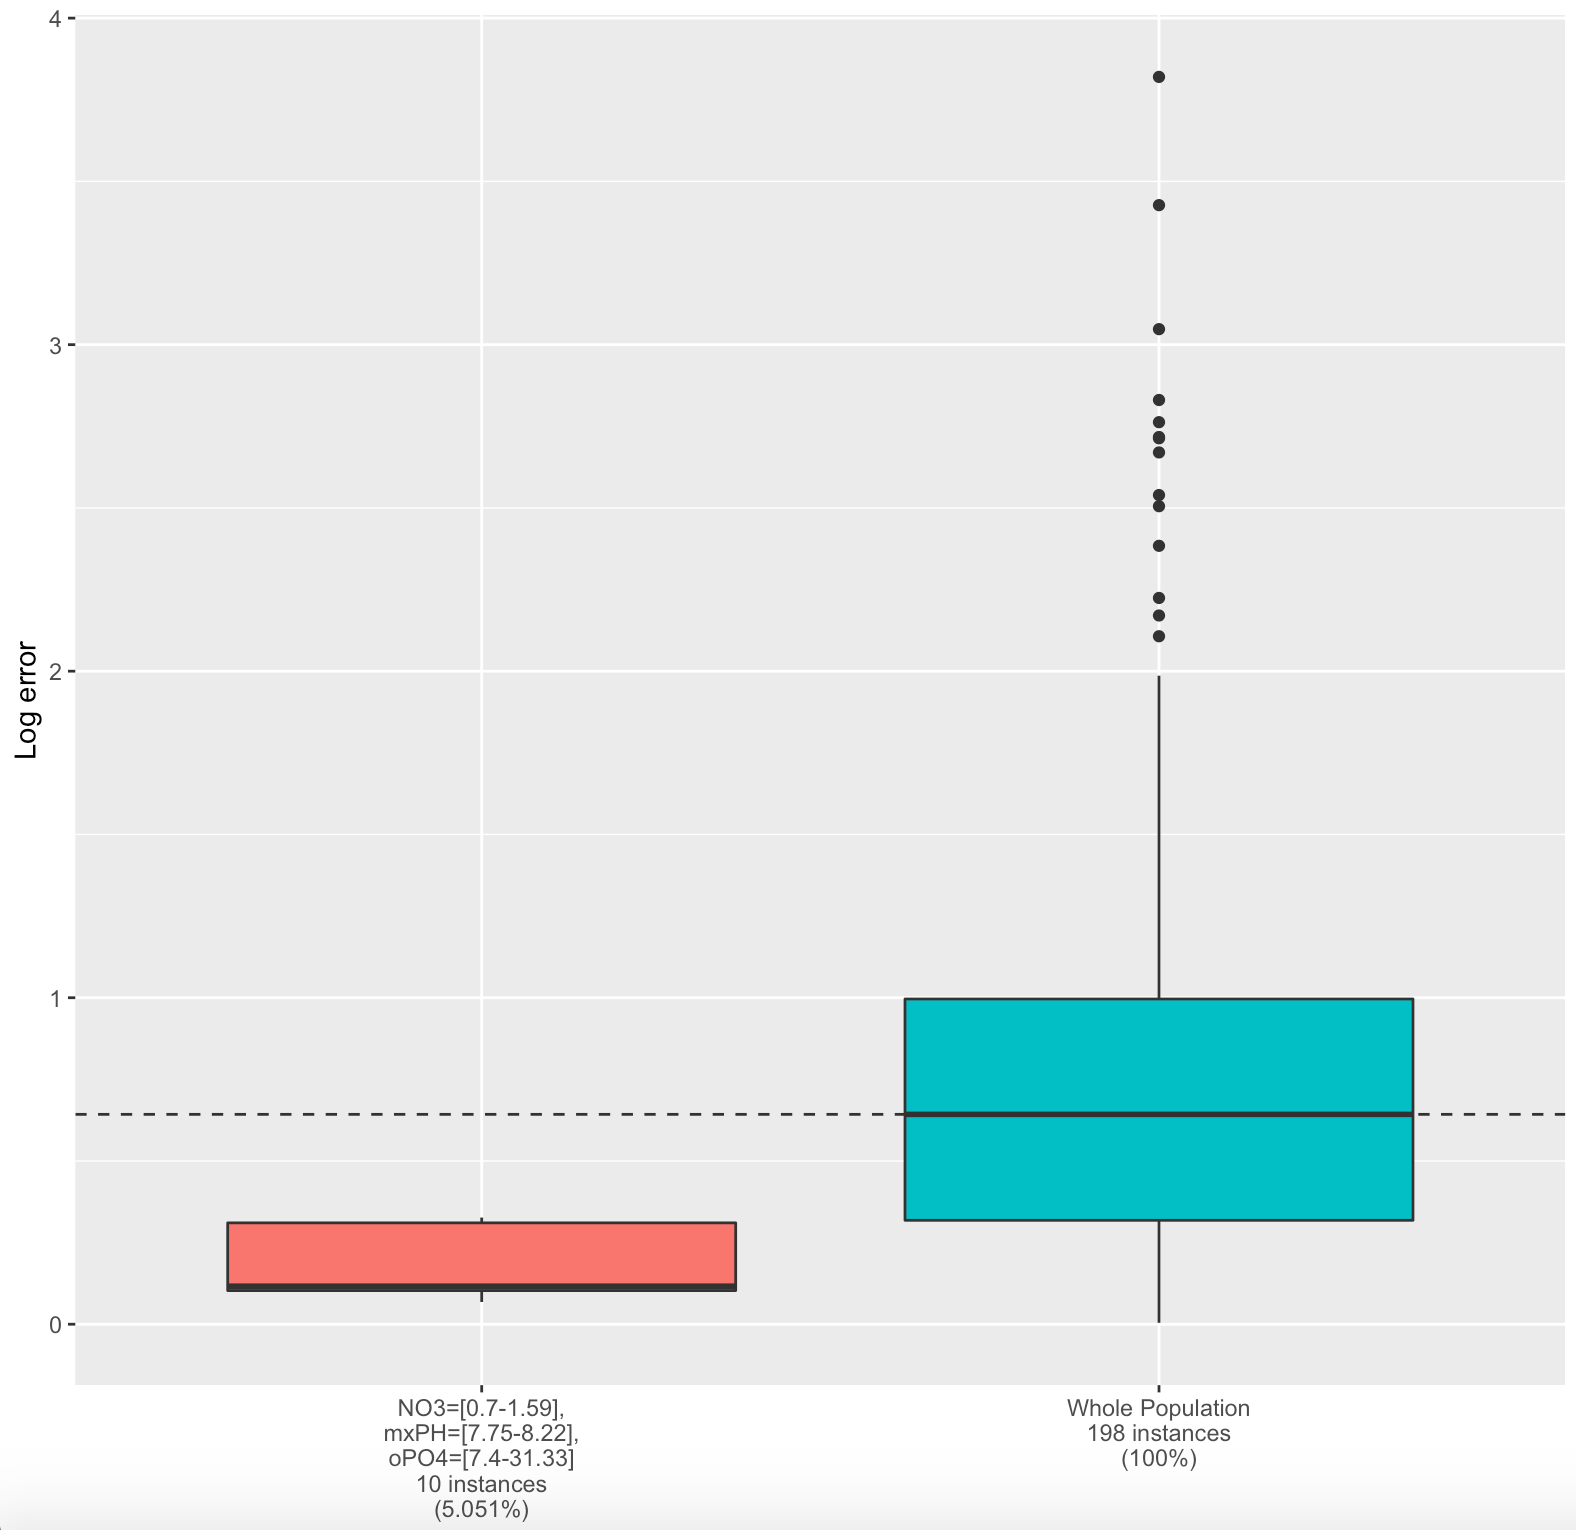
\includegraphics[width=0.45\textwidth]{/chpt_4/boxplot/single.png}
 	\caption[Caption.]
 	{Caption.}
 	\label{fig:boxplot_single}
\end{figure}

Figure \ref{fig:fig_2} contains an example of subfigures (Figure \ref{fig:subfigure_1}, ...).

\begin{figure}[!htb]
\centering
\imagewidth=0.32\textwidth
\captionsetup[subfigure]{width=0.8\imagewidth}
\begin{subfigure}{.32\textwidth}
  \centering
  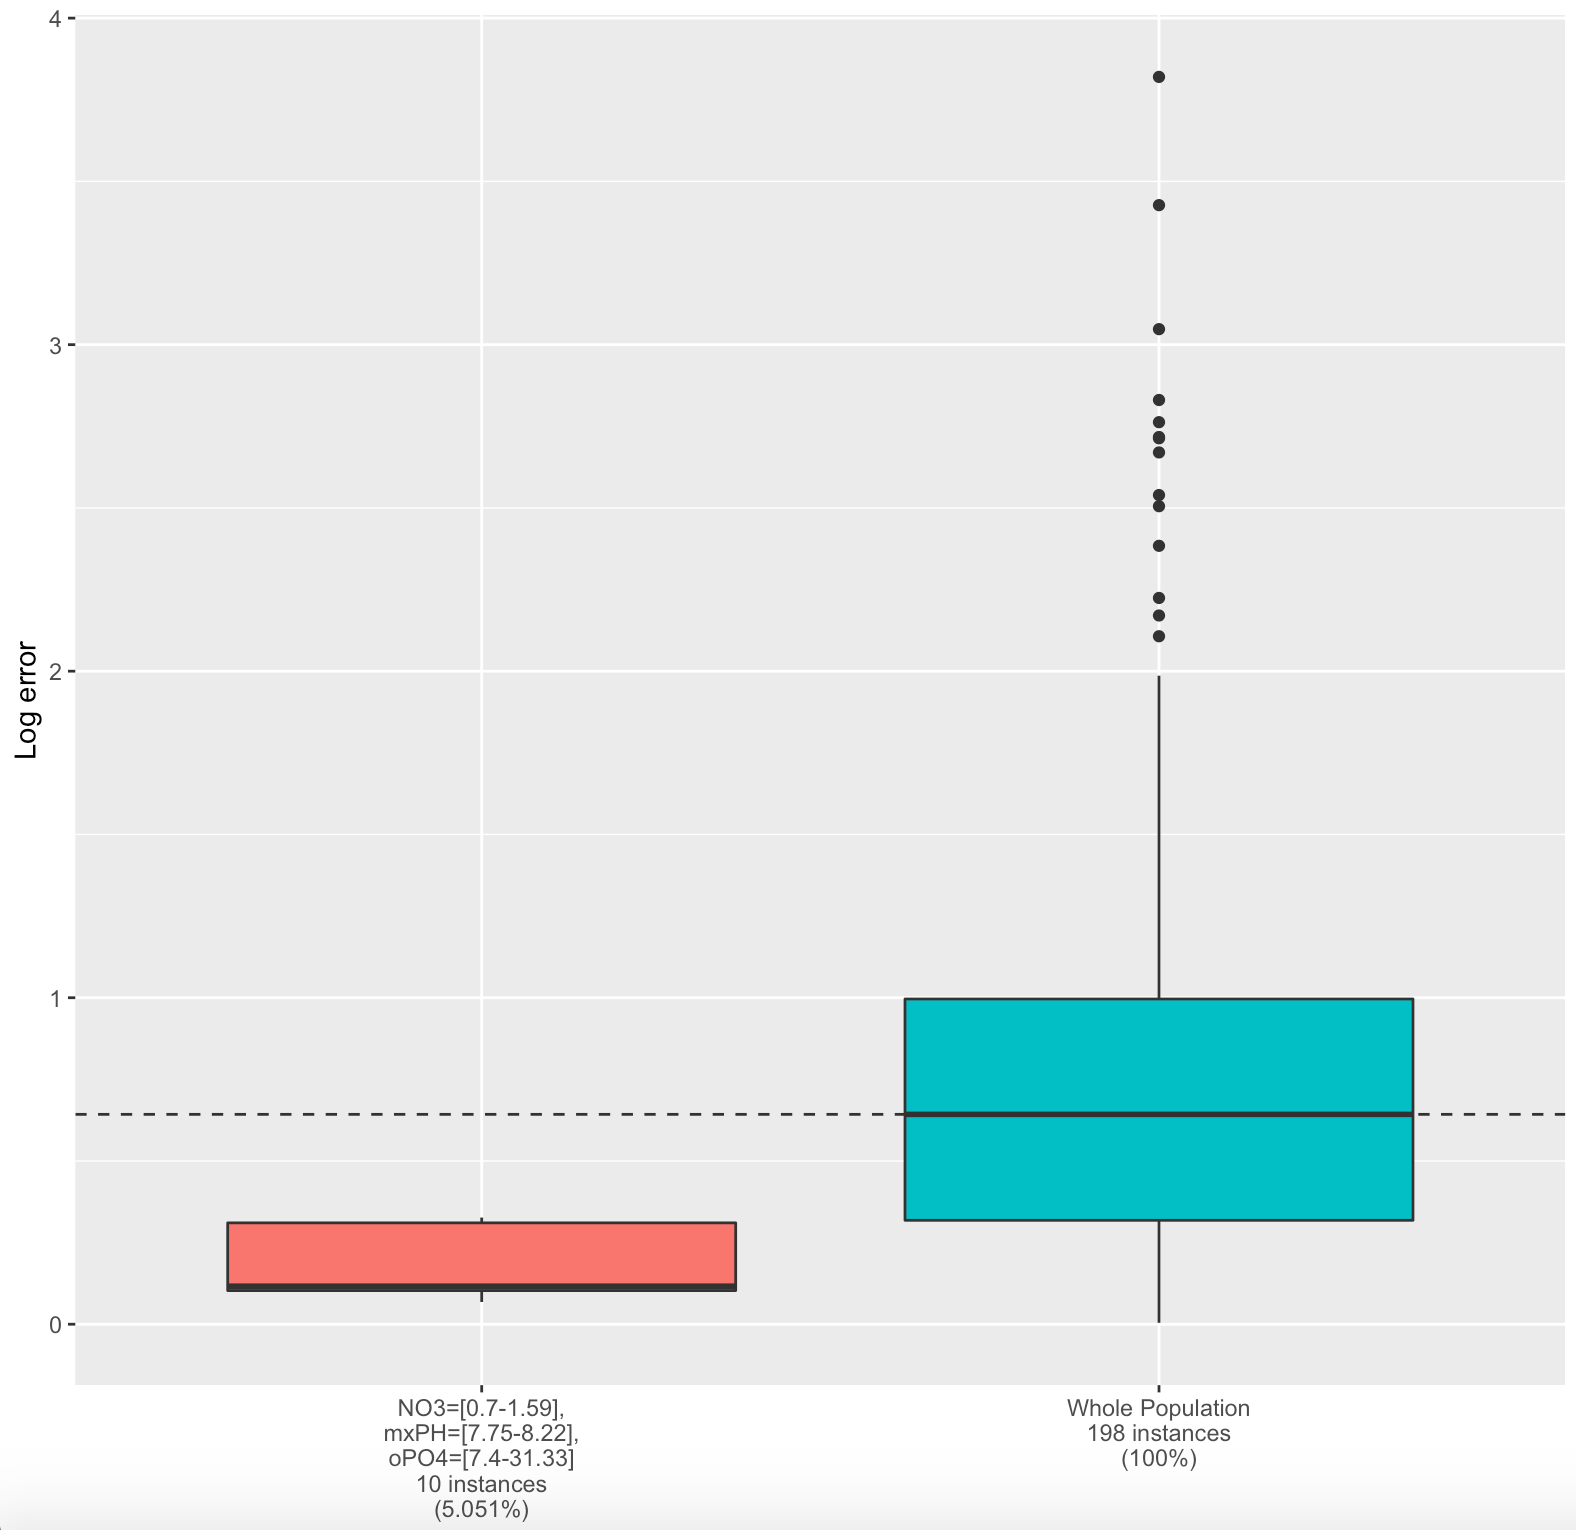
\includegraphics[width=0.97\linewidth]{/chpt_4/boxplot/single.png}
  \caption{Caption.}
  \label{fig:subfigure_1}
\end{subfigure}
\begin{subfigure}{.32\textwidth}
  \centering
  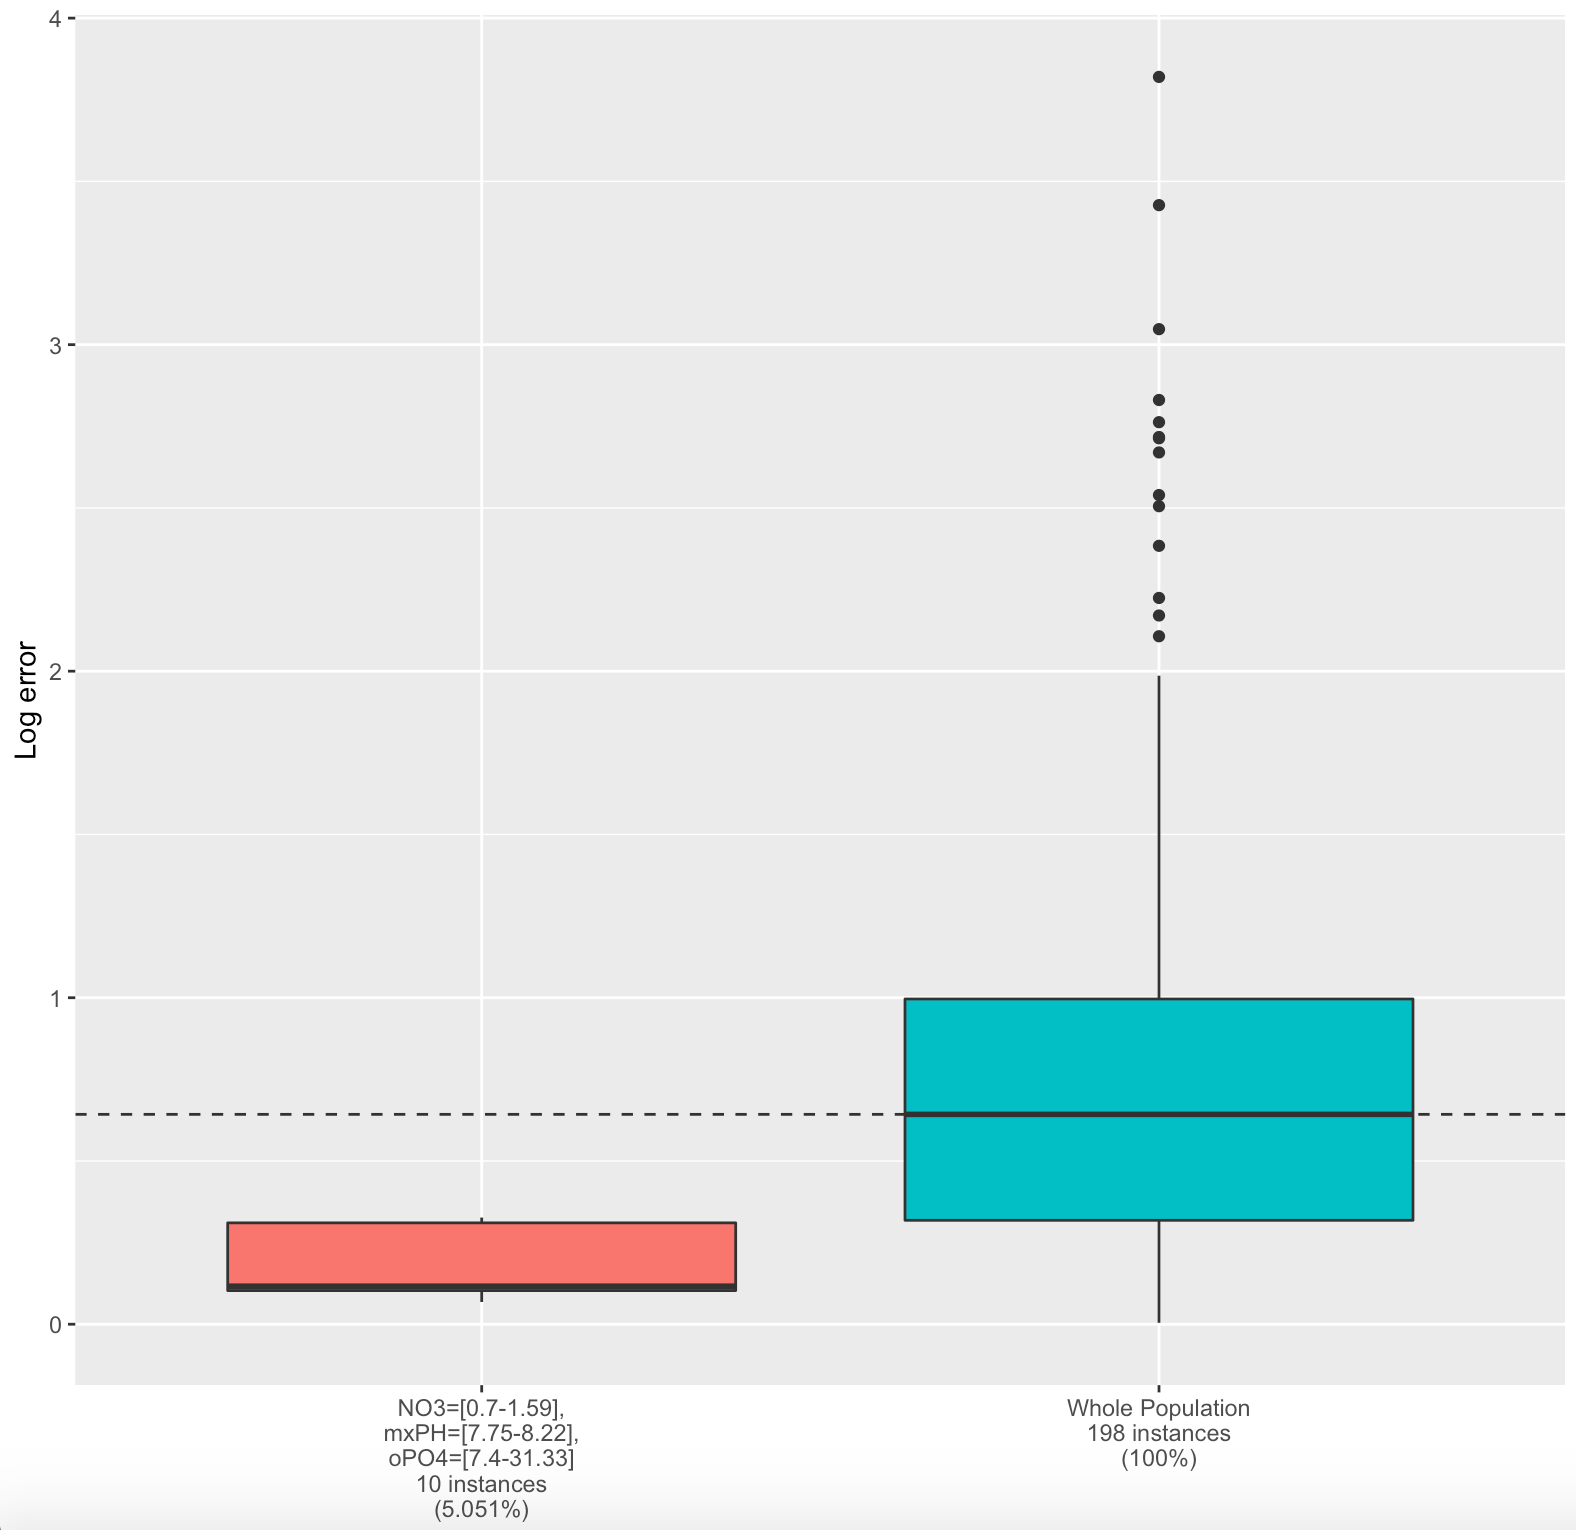
\includegraphics[width=0.97\linewidth]{/chpt_4/boxplot/single.png}
  \caption{Caption.} 
  \label{fig:subfigure_2}
\end{subfigure}
\begin{subfigure}{.32\textwidth}
  \centering
  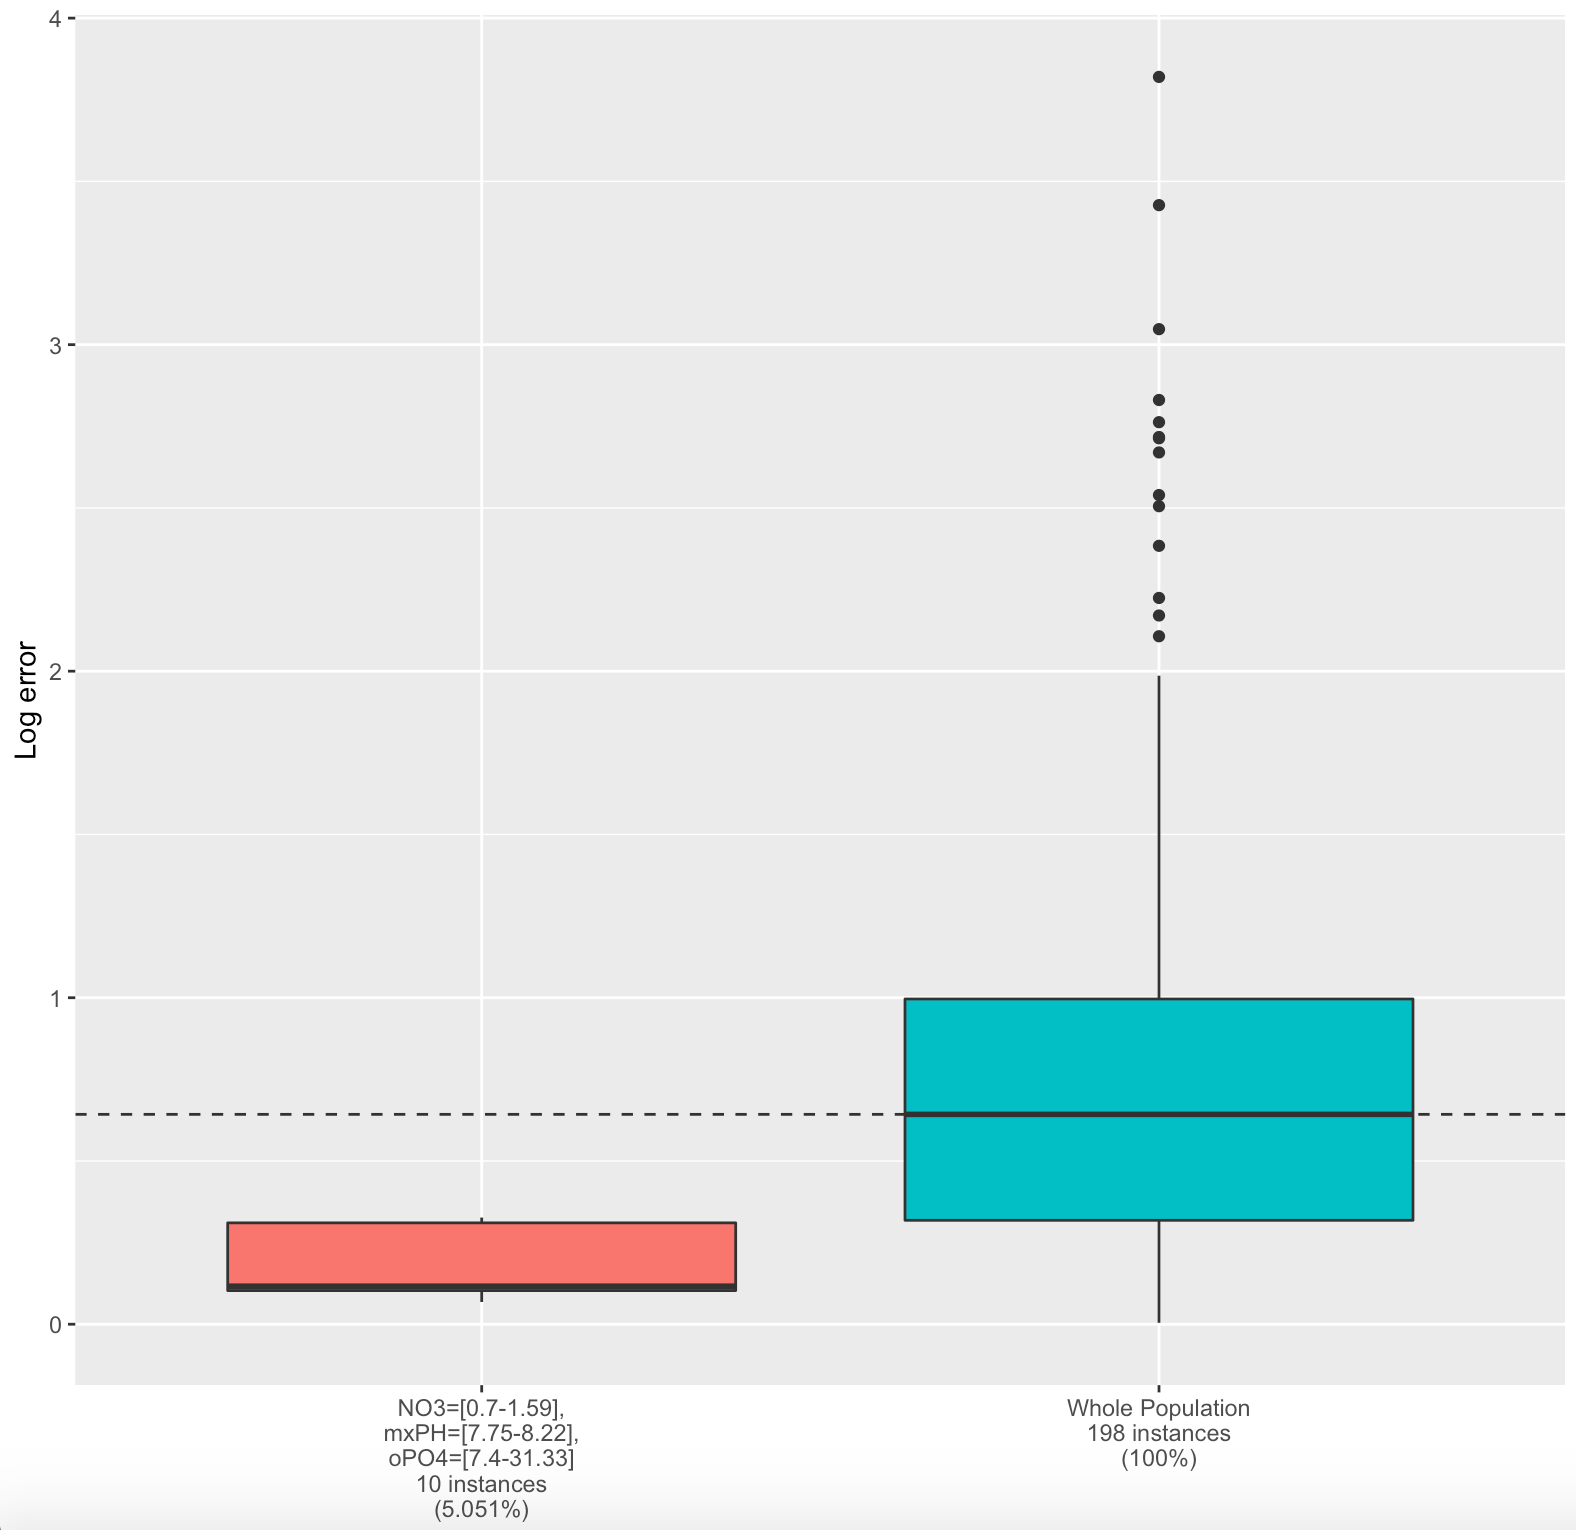
\includegraphics[width=0.97\linewidth]{/chpt_4/boxplot/single.png}
  \caption{Caption.} 
  \label{fig:subfigure_3}
\end{subfigure}
\caption{Caption.}
\label{fig:fig_2}
\end{figure}

\section{Summary}

Summary of the Chapter
		
	\chapter{Case Study}
\label{chap:chap5}

In this chapter, ....

\section{Motivation}

Text

\section{Dataset}

Text

\section{Methodology}

Text

Example of Listing: Listing \ref{lst:cf_case_study_2} ...
\begin{lstlisting}[label={lst:cf_case_study_2}, caption={Caption.},frame=tb, basicstyle=\footnotesize]

Something here
	
\end{lstlisting}	
		
\subsection{Overall Analysis of the Experimental Results}

Text

\section{Summary}

Summary of the Chapter
	%\clearemptydoublepage
%	
	\chapter{Conclusions and Future Work}
\label{chap:chap6}

Text
	
	
	
	
	\bibliography{chapters/references.bib}
	
	
	\begin{appendices}

\chapter{Title}
\label{appendix_A}



\end{appendices}

	
	
	%\chapter{Anexos}
\label{chap:chap7}



	%\clearemptydoublepage
\end{document}